% !Mode:: "TeX:UTF-8"
\chapter{系统总体设计}
\label{chapter-general_design}

\section{系统总体架构}
系统总体架构分两层,底层框架层和上层应用层,如图\ref{structure}。
\begin{figure}[h!]
    \centering
    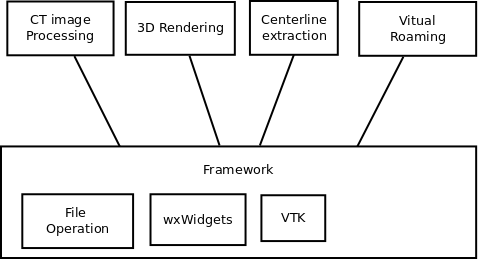
\includegraphics[width=350bp]{figure/structure.png}
    \caption{系统总体架构图}
    \label{structure}
\end{figure}

底层框架层:包含文件操作类,图形界面库wxWidgets和VTK库用来进行高效的渲染。上层应用类使用底层框架提供的功能,实现具体功能。下面分模块阐释:
\subsection{CT图像处理}

